\documentclass{article}
\usepackage[utf8]{inputenc}
\usepackage[spanish]{babel}
\usepackage{listings}
\usepackage{hyperref}
\usepackage{multirow}
\usepackage{graphicx}
\usepackage{amsmath}
\usepackage{graphicx}
\usepackage{fancyhdr}
\usepackage{geometry}
\usepackage{array}
\usepackage{float}
\usepackage{xcolor}
\geometry{a4paper, margin=1in}
\usepackage{booktabs} % Para líneas más bonitas en las tablas

%Aumentar el tamaño de fuente
\renewcommand{\normalsize}{\fontsize{12}{14}\selectfont}


% Información reutilizable
\newcommand{\myTitle}{Teoría del tema 2: Existencias: Compras y Ventas}
\newcommand{\myAuthor}{Ismael Sallami Moreno}
\newcommand{\myDegree}{Doble Grado Ingeniería Informática y Administración y Dirección de Empresas}
\newcommand{\mySubject}{Contabilidad Financiera I}
\newcommand{\myDate}{\today}

% cambiando la fuente

\begin{document}

% Portada
\begin{titlepage}
    \centering
    \begin{minipage}{0.45\textwidth}
        \centering
        
\includegraphics[width=0.8\textwidth]{../images/logo_ugr.jpg}
    \end{minipage}    \hfill
    \begin{minipage}{0.45\textwidth}
        \centering
        
\includegraphics[width=0.8\textwidth]{../images/logo_economicas.jpg} 
    \end{minipage}
    \vspace{1cm}
    
    {\scshape\LARGE \myDegree \par}
    \vspace{1cm}
    {\scshape\Large \mySubject \par}
    \vspace{1.5cm}
    {\huge\bfseries \myTitle \par}
    \vspace{2cm}
    {\Large\itshape \myAuthor \par}
    \vfill
    \myDate\par
\end{titlepage}

\tableofcontents
\newpage

\section{INTRODUCCIÓN}

El objetivo principal de esta unidad didáctica consiste, en primer lugar, en conocer que se entiende por existencias, analizar sus principales características y tipología. A continuación, se establecen cuáles son los criterios de valoración de entrada de estas existencias, así como los criterios de asignación de valor de las mismas con el fin de determinar el coste de las ventas y el valor de las existencias finales. Se realiza una primera toma de contacto con la Norma de valoración 14 del PGC sobre los ingresos por ventas y prestación de servicios, así como sobre la contabilización del impuesto de valor añadido. Por último, se analizan una serie de operaciones vinculadas a las existencias y se hace referencia a cómo se presenta en las Cuentas Anuales la información relativa a las mismas.

\section{2.1. EXISTENCIAS: CONCEPTO, CARACTERÍSTICAS Y TIPOLOGÍA}

El Plan General de Contabilidad (PGC) define las existencias en la misma línea que la Norma Internacional de Contabilidad 2 (Existencias), NIC 2.

\begin{itemize}
    \item Las existencias son activos poseídos para:
    \begin{itemize}
        \item Ser vendidos en el curso normal de las operaciones de explotación.
        \item Incorporarse al proceso de producción.
        \item Ser consumidos en el proceso de producción o en la prestación de servicios.
    \end{itemize}
    \item Así, se diferencian tres tipos de existencias según el destino de las mismas:
    \begin{itemize}
        \item Activos poseídos para su venta sin transformación.
        \item Activos poseídos para transformar.
        \item Activos poseídos para utilizar en cualquier fase del proceso de transformación de bienes y servicios.
    \end{itemize}
\end{itemize}


Los subgrupos y cuentas relativas a las existencias contempladas en el PGC son los que se detallan en la figura 1.

\begin{figure}[H]
    \centering
    \begin{tabular}{|p{4cm}|p{4cm}|p{4cm}|}
        \hline
        \textbf{Tipo de existencia} & \textbf{Subgrupo} & \textbf{Cuenta} \\
        \hline
        \multirow{3}{*}{\rotatebox{90}{\parbox{2cm}{Adquiridas del exterior}}} & 30. Comerciales & 300. Mercaderías \\
        \cline{2-3}
        & 31. Materias Primas & 310. Materias primas \\
        \cline{2-3}
        & \multirow{6}{*}{32. Otros aprovisionamientos} & 320. Elementos y conjuntos incorporables \\
        \cline{3-3}
        & & 321. Combustible \\
        \cline{3-3}
        & & 322. Repuestos \\
        \cline{3-3}
        & & 325. Materiales Diversos \\
        \cline{3-3}
        & & 326. Embalajes \\
        \cline{3-3}
        & & 327. Envases \\
        \cline{3-3}
        & & 328. Material de Oficina \\
        \hline
        \multirow{5}{*}{\rotatebox{90}{\parbox{2cm}{Surgidas del proceso productivo}}} & 33. Productos en curso & 330. Productos en curso \\
        \cline{2-3}
        & 34. Productos semiterminados & 340. Productos semiterminados \\
        \cline{2-3}
        & 35. Productos terminados & 350. Productos terminados \\
        \cline{2-3}
        & 36. Subproductos, residuos y materiales recuperados & 360. Subproductos \\    \cline{3-3}
        & & 365. Residuos \\
        \cline{3-3}
        & & 368. Material recuperado \\
        \hline
    \end{tabular}
    \caption{Subgrupos y cuentas del PGC relacionadas con las existencias}
\end{figure}

El subgrupo 30 es propio de las empresas comerciales, es decir, las adquiridas del exterior que no requieren de un proceso de modificación física o fabricación en la empresa, y los subgrupos 31, 33, 34, 35, 36 y la cuenta 320 son propios de las empresas industriales, donde sí se produce un proceso de modificación de las materias inicialmente adquiridas e incluidas en un proceso de fabricación, mientras que el resto de los subgrupos pueden ser compartidos por cualquier empresa. A continuación, la figura 2 incluye las definiciones de los distintos subgrupos, según indica el PGC en su segunda parte:

\begin{figure}[h]
    \centering
    \begin{tabular}{|m{2cm}|m{3cm}|m{6cm}|}
        \hline
        \textbf{Subgrupo} & \textbf{Denominación} & \textbf{Definición} \\
        \hline
        30 & Comerciales & Bienes adquiridos por la empresa y destinados a la venta sin transformación. \\
        \hline
        31 & Materias primas & Las que, mediante elaboración o transformación, se destinan a formar parte de los productos fabricados. \\
        \hline
        32 & (320) Elementos y conjuntos incorporables & Los fabricados normalmente fuera de la empresa y adquiridos por ésta para incorporarlos a su producción sin someterlos a transformación. \\
        \hline
    \end{tabular}
    \caption{Tipología de existencias, subgrupo y definición}
\end{figure}

\section*{Existencias no sometidas a transformación}

\begin{tabular}{|p{4cm}|p{4cm}|p{4cm}|}
\hline
\textbf{Subgrupo} & \textbf{Denominación} & \textbf{Definición} \\
\hline
32 & (321) Combustibles & Materias energéticas susceptibles de almacenamiento. \\
\hline
32 & (322) Repuestos & Piezas destinadas a ser montadas en instalaciones, equipos o máquinas en sustitución de otras semejantes. Se incluirán en esta cuenta las que tengan un ciclo de almacenamiento inferior a un año. \\
\hline
32 & (325) Materiales diversos & Otras materias de consumo que no han de incorporarse al producto fabricado. \\
\hline
32 & (326) Embalajes & Cubiertas o envolturas, generalmente irrecuperables, destinadas a resguardar productos o mercaderías que han de transportarse. \\
\hline
32 & (327) Envases & Recipientes o vasijas, normalmente destinadas a la venta juntamente con el producto que contienen. \\
\hline
32 & (328) Material de oficina & El destinado a la finalidad que indica su denominación, salvo que la empresa opte por considerarlo que el material de oficina adquirido durante el ejercicio es objeto de consumo en el mismo. \\
\hline
\end{tabular}

\section*{Existencias sometidas a transformación}

\begin{tabular}{|p{4cm}|p{4cm}|p{4cm}|}
\hline
\textbf{Subgrupo} & \textbf{Denominación} & \textbf{Definición} \\
\hline
33 & Productos en curso & Bienes o servicios que se encuentran en fase de formación o transformación en un centro de actividad al cierre del ejercicio y que no deban registrarse en las cuentas de los subgrupos 34 o 36. \\
\hline
34 & Productos semiterminados & Los fabricados por la empresa y no destinados normalmente a su venta hasta tanto sean objeto de elaboración, incorporación o transformación posterior. \\
\hline
35 & Productos terminados & Los fabricados por la empresa y destinados al consumo final o a su utilización por otras empresas. \\
\hline
36 & (360) Subproductos & Los de carácter secundario o accesorio de la fabricación principal. \\
\hline
36 & (365) Residuos & Los obtenidos inevitablemente y al mismo tiempo que los productos o subproductos, siempre que tengan valor intrínseco y puedan ser utilizados o vendidos. \\
\hline
36 & (368) Materiales recuperables & Los que, por tener valor intrínseco, entran nuevamente en almacén después de haber sido utilizados en el proceso productivo. \\
\hline
\end{tabular}

\section*{}

Un caso que requiere una mención especial, y que se recoge en el epígrafe 2.4.8 del presente capítulo, es la incorporación del concepto de prestación de servicios en las existencias, registrándolos al coste de producción siempre que no se hayan reconocido los ingresos correspondientes a los mismos.

\section{Reconocimiento y Valoración Inicial de las Existencias}

Uno de los aspectos más importantes de las existencias se refiere a su valoración por el efecto que esto ocasiona en la situación patrimonial y en la cuenta de resultados de la empresa. En este sentido, resulta necesario, en primer lugar, establecer un marco general de valoración de estas existencias, donde se establezcan, principalmente, las diferencias en cuanto a su forma de adquisición, así como, el criterio de valoración de las entradas, y el método de asignación de valor de las salidas, el cual se encuentra recogido en la figura 3.

\begin{figure}[H]
    \centering
    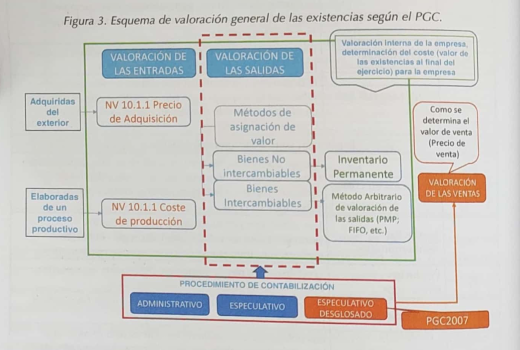
\includegraphics[width=\textwidth]{figura3.png}
    \caption{Esquema de valoración general de las existencias según el PGC.}
\end{figure}

\subsection{Valoración de las Entradas}
\begin{itemize}
    \item Adquiridas del exterior
    \begin{itemize}
        \item NV 10.1.1 Precio de Adquisición
    \end{itemize}
    \item Elaboradas de un proceso productivo
    \begin{itemize}
        \item NV 10.1.1 Coste de producción
    \end{itemize}
\end{itemize}

\subsection{Valoración de las Salidas}
\begin{itemize}
    \item Métodos de asignación de valor
    \begin{itemize}
        \item Bienes No Intercambiables
        \item Bienes Intercambiables
    \end{itemize}
    \item Inventario Permanente
    \begin{itemize}
        \item Método Arbitrario de valoración de las salidas (PMP, FIFO, etc.)
    \end{itemize}
\end{itemize}

\subsection{Valoración de las Ventas}
\begin{itemize}
    \item Valoración Interna de la empresa, determinación del coste (valor de las existencias al final del ejercicio) para la empresa
    \item Cómo se determina el valor de venta (Precio de venta)
\end{itemize}

\subsection{Procedimiento de Contabilización}
\begin{itemize}
    \item Administrativo
    \item Especulativo
    \item Especulativo Desglosado
\end{itemize}

\subsection{Valoración de las entradas de existencias}

Partiendo del esquema presentado en la figura 3, la NV 10 señala que los bienes y servicios comprendidos en las existencias se valorarán por su coste, ya sea el precio de adquisición o el coste de producción, ya sean adquiridos en el exterior o producidos por la empresa, respectivamente.

\subsubsection{Precio de adquisición de las existencias}

Concretamente, el precio de adquisición está formado por el importe facturado por el proveedor más todos los gastos adicionales que se produzcan hasta que los bienes se encuentren ubicados para su venta, tales como transportes, aranceles de aduanas, seguros y otros directamente atribuibles a la adquisición de existencias.

Los impuestos indirectos que gravan las existencias solo se incluirán en el precio de adquisición o coste de producción cuando no sean recuperables directamente de la Hacienda Pública (NV10 PGC).

En concreto, los gastos adicionales son:
\begin{itemize}
    \item Transportes, fletes y comisiones con cargo al comprador.
    \item Seguro, depósito y custodia en tránsito.
    \item Impuestos satisfechos por la compra no recuperables, incluidos aranceles y otros derechos.
    \item Inspección y conservación, si son por cuenta del comprador.
\end{itemize}

En las existencias que necesiten un periodo de tiempo superior a un año para estar en condiciones de ser vendidas, se incluirán en el precio de adquisición o coste de producción, los gastos financieros, en la medida en que se devenguen hasta el momento de inmovilizado material.

Del importe facturado por el proveedor se deducirá cualquier descuento, rebaja o bonificación y otras partidas similares, como los intereses incorporados al nominal de las deudas por adquisición en condiciones de aplazamiento, incluidos los no comerciales o financieros.

A modo de esquema, la valoración inicial incluiría:

\textbf{Figura 4. Esquema de valoración general de las existencias según el PGC}

\begin{itemize}
    \item PRECIO DE COMPRA/FACTURA
    \begin{itemize}
        \item Importe facturado
        \item (-) Descuentos y rebajas
    \end{itemize}
    \item (+) Impuestos no recuperables (NV.10.1) no recuperables:
    \begin{itemize}
        \item Gastos financieros (si se devengan hasta el momento de inmovilizado material NV.10.1)
        \item Seguros, depósitos y custodia en tránsito
        \item Inspección y conservación
    \end{itemize}
    \item (+) OTROS GASTOS ADICIONALES:
    \begin{itemize}
        \item Transporte
        \item Aranceles y otros impuestos no recuperables directamente de la Hacienda Pública
        \item Comisiones con cargo al comprador
        \item Otros gastos directamente atribuibles hasta que los bienes se hallen ubicados para su venta
    \end{itemize}
\end{itemize}

\section*{Ejemplo 1}

Una empresa adquiere 800 unidades de una mercancía a un precio unitario de 75 €. Además, se obtiene un descuento comercial de 2.000 € y un descuento por pronto pago fuera de factura de 200 €. Los aranceles de la aduana ascienden a 600 €. La empresa incurre en unos gastos de transporte de la mercancía hasta su almacén por importe de 5.000 € y de seguro por importe de 2.000 €. El proveedor concede un descuento de 500 € en el caso de que se superen las 3.000 unidades de compra al año. Los costes de administración y almacenamiento de las mercancías ascienden a 1.600 €.

\section*{Solución}

Veamos el proceso de cálculo del precio de adquisición en base a la normativa contable anteriormente.

\begin{align*}
\text{Importe de la adquisición (800 unidades al precio de 75 €)} &= 60.000 € \\
\text{- Descuento comercial} &= -2.000 € \\
\text{+ Aranceles} &= +600 € \\
\text{+ Gastos de transporte} &= +5.000 € \\
\text{+ Seguros} &= +2.000 € \\
\text{Precio de Adquisición} &= 65.600 €
\end{align*}

\subsubsection{Coste de producción de las existencias}

El coste de producción de las existencias en una empresa industrial se determina sumando al precio de adquisición de las materias primas y otras materias consumibles, los costes directamente imputables al producto. También se incluyen los costes indirectos atribuibles al producto.

El coste de estos productos se valora aplicando el criterio del coste de producción, que se usa para valorar las existencias de productos terminados, productos semiterminados, y productos en curso.

Los elementos que forman el coste de producción son los siguientes:

\begin{itemize}
    \item \textbf{Costes directos:} Incluyen el precio de adquisición de la materia prima y otras materias consumibles, así como los costes directamente imputables al producto, como la mano de obra directa.
    \item \textbf{Costes indirectos:} Son aquellos que no se pueden identificar directamente en los productos y requieren criterios de reparto para determinar la parte correspondiente a cada producto. Ejemplos de estos costes son los derivados de la utilización de la capacidad normal de trabajo de los medios de producción.
\end{itemize}

Es importante considerar también los anticipos a proveedores, que afectan al concepto de existencias en la cuenta de suministros futuros de existencias y se valorarán al coste. Los débitos por operaciones comerciales se valorarán de acuerdo con la norma relativa a instrumentos financieros.

\subsection{Métodos de asignación de valor}

De acuerdo con la NV. 10.1.3, se pueden utilizar diferentes métodos de asignación de valor de las existencias según sean intercambiables o no. Los bienes no intercambiables son aquellos que son fácilmente distinguibles del resto. Cuando una empresa produce o comercializa bienes no intercambiables, se asigna valor identificando el precio o costos específicos de cada bien individualmente.

Para bienes intercambiables, se usa generalmente el método del precio medio o coste medio ponderado. El método FIFO es aceptable si es más conveniente para la gestión de la empresa. Es importante que se mantenga un único método de asignación de valor para todas las existencias con naturaleza y uso similares, siguiendo el principio de uniformidad del PGC.

\subsubsection{Precio Medio Ponderado o Coste Medio Ponderado}
Este criterio consiste en la realización de una valoración homogénea de todos los artículos del almacén. El valor de coste de la venta es la media ponderada de los distintos precios de entrada en función del volumen de unidades adquiridas a cada uno de los precios, tal y como puede apreciarse en la siguiente fórmula.

\begin{equation}
\text{Cálculo del Precio o Coste Medio Ponderado} = \frac{(q_1 \times p_1) + (q_2 \times p_2) + \ldots + (q_n \times p_n)}{q_1 + q_2 + \ldots + q_n}
\end{equation}

Donde, $q$ es la cantidad de producto adquirido, y $p$ es el precio al que fue adquirido el producto $n$.

\subsubsection{FIFO (First in first out, Primera Entrada - Primera salida)}
El coste de la venta será el más antiguo de los precios de adquisición existentes, y las existencias finales coincidirán con las últimas entradas en el almacén de mercancías.

Veamos el siguiente ejemplo de valoración de las salidas, utilizando la ficha de inventario.

\section*{Ejemplo 2.2}

Una empresa comercial presenta los siguientes movimientos de almacén del producto X para el mes de enero del ejercicio económico 2020.

\begin{table}[h]
\centering
\caption{Movimientos de almacén del producto X}
\begin{tabular}{llll}
\toprule
Concepto & Fecha & Unidades & Precio unitario \\
\midrule
Existencia inicial & 1 de enero & 300 & 2 \\
Compra & 10 de enero & 500 & 2.5 \\
Venta & 15 de enero & 400 &  7 \\
Compra & 20 de enero & 400 & 3 \\
Venta & 25 de enero & 600 & 15 \\
\bottomrule
\end{tabular}
\end{table}

\textbf{SE PIDE:} Determinar el coste de las ventas y realizar la valoración de las existencias finales, aplicando el criterio PMP y FIFO.

\subsection*{Solución}

En primer lugar, planteamos la solución del ejercicio siguiendo el criterio del PMP.

\subsubsection*{Criterio PMP}

Como se ha comentado en la exposición teórica, el PMP busca obtener un precio medio ponderado para hacer la valoración del coste de las salidas. En este sentido, conforme se van añadiendo diferentes existencias con diferentes costes, es necesario calcular este nuevo precio ponderado. En la tabla siguiente, el primer cálculo del PMP se produce cuando se realiza la primera compra del 10 de enero.

En ese momento tenemos dos precios distintos, el precio de compra de esta misma fecha y el precio de las existencias iniciales, por lo que hay que calcular el precio medio ponderado. La siguiente fecha donde hay que volver a calcular este nuevo precio es el 20 de enero, en ese momento, se produce la adquisición de un nueva tipo de existencia a otro precio distinto. La adquisición de nuevas compras de existencias con precios distintos cambia el precio medio ponderado, tal y como puede apreciarse en la columna existencias, en las fechas a las que hemos hecho referencia.

\section*{Ejemplo 2}

Una empresa comercial presenta los siguientes movimientos de almacén del producto X para el mes de enero del ejercicio económico 2020:

\begin{tabular}{|c|c|c|c|}
\hline
\textbf{Concepto} & \textbf{Fecha} & \textbf{Unidades} & \textbf{Precio unitario} \\
\hline
Existencia inicial & 1 de enero & 300 & 2 \\
\hline
Compra & 10 enero & 500 & 2,5 \\
\hline
Venta & 15 enero & 400 & 7 \\
\hline
Compra & 20 enero & 400 & 3 \\
\hline
Venta & 25 enero & 600 & 15 \\
\hline
\end{tabular}

\subsection*{SE PIDE}
Determinar el coste de las ventas y realizar la valoración de las existencias finales, aplicando el criterio PMP y FIFO.

\subsection*{PMP}
\textbf{Solución}

En primer lugar, planteamos la solución del ejercicio siguiendo el criterio del Precio Medio Ponderado (PMP).

\section*{Criterio PMP}

Como se ha comentado en la exposición teórica, el PMP busca obtener un precio medio ponderado para hacer la valoración del coste de las salidas. Conforme se van añadiendo diferentes existencias con diferentes costes es necesario calcular este nuevo precio ponderado. En la tabla siguiente, el primer cálculo del PMP se produce cuando se realiza la primera compra del 10 de enero. En ese momento tenemos dos precios distintos: el precio de compra de esta misma fecha y el precio de las existencias iniciales, por lo que hay que calcular el precio medio ponderado. La siguiente fecha donde hay que volver a calcular este nuevo precio es el 20 de enero, cuando se produce la adquisición de un nuevo tipo de existencia a otro precio distinto. La adquisición de nuevas compras de existencias con precios distintos cambia el precio medio ponderado, tal y como puede apreciarse en la columna existencias, en las fechas a las que hemos hecho referencia.

\begin{table}[H]
    \centering
    \begin{tabular}{|c|ccc|ccc|ccc|}
    \hline
    \textbf{FECHA} & \multicolumn{3}{c|}{\textbf{ENTRADAS}} & \multicolumn{3}{c|}{\textbf{SALIDAS}} & \multicolumn{3}{c|}{\textbf{EXISTENCIAS}} \\
    \hline
     & \textbf{U} & \textbf{P} & \textbf{CT} & \textbf{U} & \textbf{P} & \textbf{CT} & \textbf{U} & \textbf{P} & \textbf{CT} \\
    \hline
    1/1 & 300 & 2 & 600 &  &  &  & 300 & 2 & 600 \\
    \hline
    10/1 & 500 & 2.5 & 1,250 &  &  &  & 300 &  &  \\
     &  &  &  &  &  &  & 500 & 2.3125 & 1,850 \\
     &  &  &  &  &  &  & 800 &  &  \\
    \hline
    15/1 &  &  &  & 400 & 2.3125 & 925 & 400 & 2.3125 & 925 \\
     &  &  &  &  &  &  & 400 &  &  \\
     &  &  &  &  &  &  & 800 &  &  \\
    \hline
    20/1 & 400 & 3 & 1,200 &  &  &  & 400 & 2.65625 & 2,125 \\
     &  &  &  &  &  &  & 400 &  &  \\
     &  &  &  &  &  &  & 800 &  &  \\
    \hline
    25/1 &  &  &  & 600 & 2.65625 & 1,594 & 200 & 2.65625 & 531 \\
    \hline
    \textbf{TOTAL} & 3,050 & 1,000 &  & 2,519 &  &  & 531 &  &  \\
    \hline
    \end{tabular}
\end{table}
    
    
    
Donde U son unidades, P es el precio y CT es el coste total.

\[
\text{PMP (10/1)} = \frac{600 + 1,250}{800} = 2.3125\]
\[\text{PMP (20/1)} = \frac{925 + 1,200}{800} = 2.65625
\]

\[
\text{Existencias finales (200 unidades)} = 531 \, \text{€}
\]
\[
\text{Coste de las ventas (1,000 unidades)} = 2,519 \, \text{€} \, (925 + 1,594)
\]

Cuando se producen las ventas en este supuesto, el 15 de enero y el 25 de enero, la empresa sabe que el coste de las mismas es de 2.31 € y de 2.65 €, respectivamente. Esto se traduce en que si la empresa quiere tener un beneficio contable siguiendo este criterio, el precio de venta por unidad debe ser superior a estos importes.

\section*{Solución Aplicando FIFO}

\section*{Criterio FIFO}

\textbf{Veamos a continuación cual sería la solución si aplicamos el criterio FIFO.}
\begin{table}[H]
    \centering
    \begin{tabular}{|c|ccc|ccc|ccc|}
    \hline
    \textbf{FECHA} & \multicolumn{3}{c|}{\textbf{ENTRADAS}} & \multicolumn{3}{c|}{\textbf{SALIDAS}} & \multicolumn{3}{c|}{\textbf{EXISTENCIAS}} \\
    \hline
     & \textbf{U} & \textbf{P} & \textbf{CT} & \textbf{U} & \textbf{P} & \textbf{CT} & \textbf{U} & \textbf{P} & \textbf{CT} \\
    \hline
    1/1 & 300 & 2 & 600 &  &  &  & 300 & 2 & 600 \\
    \hline
    10/1 & 500 & 2.5 & 1,250 &  &  &  & 300 & 2 & 600 \\
     &  &  &  &  &  &  & 500 & 2.5 & 1,250 \\
     &  &  &  &  &  &  & 800 &  & 1850 \\
    \hline
    15/1 &  &  &  & 300 & 2 & 600 &  &  &  \\
     &  &  &  & 100 & 2.5 & 250 & 400 & 2.5 & 1000  \\
     &  &  &  & 400 &  & 850 &  &  &  \\
    \hline
    20/1 & 400 & 3 & 1,200 &  &  &  & 400 & 2.5 & 1000 \\
     &  &  &  &  &  &  & 400 & 3 & 1200 \\
     &  &  &  &  &  &  & 800 &  & 2250  \\
    \hline
    25/1 &  &  &  & 400 & 2.5 & 1000 &  &  &  \\
    &  &  &  & 200  & 3 & 600 & 200 & 3 & 600 \\
    &  &  &  & 600 &  & 1600 &  &  &   \\    \hline
    \textbf{TOTAL} &  & & 3050 & 1000 &  & 2450 &  &  & 600 \\
    \hline
    \end{tabular}
    \caption{\textbf{CUIDADO}: en la columna de precios, estan en medio, los he puesto asi por facilidades.}
\end{table}

Para el caso de que la empresa utilice el criterio FIFO, ahora no se debe calcular ningún precio medio entre las existencias. En su lugar, las existencias se ordenan en función de su llegada. Para el caso que nos ocupa, la valoración que se le da a las salidas de las existencias es, en primer lugar, el precio que tienen las existencias iniciales. Posteriormente, se valoran las salidas por el precio de adquisición de las compras del 10 de enero y del 20 de enero, por ese orden.

No obstante, resulta conveniente analizar cómo afectan diferentes acciones que pueden llevarse a cabo y que pueden afectar a las existencias, determinando además su impacto en su coste y en el número de unidades de su inventario. A modo de resumen de la NV 10.2, las figuras 6 y 7 recogen estas acciones y su impacto.


\begin{table}[H]
    \centering
    \begin{tabular}{|p{3cm}|p{3cm}|p{3cm}|p{3cm}|}
    \hline
    \textbf{Concepto} & \textbf{¿Afecta a la valoración de existencias?} & \textbf{Coste unitario} & \textbf{Nº Unidades} \\
    \hline
    Compra & Sí & Sí & Sí \\
    \hline
    Venta & No & No & No \\
    \hline
    Descuentos s/compras por p.p. & Sí & Sí (disminuye) & Sí (disminuye) \\
    \hline
    Transportes s/compras & Sí & Sí (aumenta) & No \\
    \hline
    Transportes s/ventas & No & No & No \\
    \hline
    Descuento comercial compras & Sí & Sí (disminuye) & No \\
    \hline
    Descuento comercial ventas & No & No & No \\
    \hline
    Devolución de compras & Sí & Sí & No \\
    \hline
    Devolución de ventas & No & No & Sí (disminuye) \\
    \hline
    Rappels por compras & Sí (depende) & Sí (disminuye) & No \\
    \hline
    \end{tabular}
    \caption{Acciones relacionadas con las existencias e impacto sobre su valoración (I) - NRV 10.2}
    \end{table}
    
    \begin{table}[H]
    \centering
    \begin{tabular}{|p{3cm}|p{3cm}|p{3cm}|p{3cm}|}
    \hline
    \textbf{Concepto} & \textbf{¿Afecta a la valoración de existencias?} & \textbf{Coste unitario} & \textbf{Nº Unidades} \\
    \hline
    Rappels sobre ventas & No & No & No \\
    \hline
    Aranceles e impuestos no repercutibles sobre compras & Sí & Sí (aumenta) & No \\
    \hline
    Subvenciones y compensaciones de compras & Sí & Sí (disminuye) & No \\
    \hline
    Otros gastos sobre compras & Sí & Sí (aumenta) & No \\
    \hline
    Gastos de venta & No & No & No \\
    \hline
    \end{tabular}
    \caption{Acciones relacionadas con las existencias e impacto sobre su valoración (II) - NRV 10.2}
    \end{table}

    \section{Valoración posterior de las existencias}


Una vez registradas las existencias según su valoración inicial, es necesario realizar una valoración posterior para establecer su valor final en las cuentas anuales al final del ejercicio. Esta nueva valoración implica ajustar el valor mediante correcciones que, en el mejor de los casos, mantendrán la valoración inicial, sin poder superarla. Estos ajustes se denominan correcciones valorativas.

Es importante diferenciar entre el deterioro de valor, que es una pérdida reversible, y la pérdida de valor definitiva, que es irreversible. Por ejemplo, el deterioro puede revertirse si se recupera el valor original, mientras que una pérdida por causas como una inundación es definitiva.
\begin{figure}[H]
    \centering
    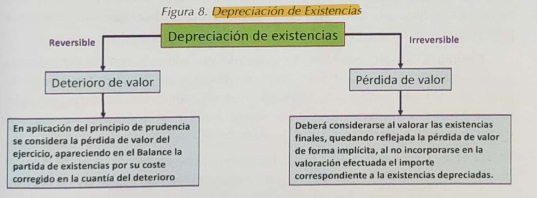
\includegraphics[width=\textwidth]{figura4.png}
\end{figure}

Cuando el valor neto realizable de las existencias es inferior al precio de adquisición o coste de producción, se deben hacer correcciones valorativas y reconocerlas como un gasto en la cuenta de pérdidas y ganancias. Si las causas de la corrección desaparecen, la corrección se revierte y se reconoce como ingreso.

El valor realizable de un activo es el importe que se puede obtener por su venta en el mercado, deduciendo los costes necesarios para la transacción y para terminar la producción si aplica.

No se realizará corrección valorativa en materias primas si los productos terminados se venderán por encima del coste. Si se requiere corrección, el precio de reposición puede ser la mejor medida. Bienes o servicios sujetos a contratos de venta no se corrigen si el precio cubre al menos el coste de las materias primas y otros costes necesarios.

\section*{Ejemplo 3}

La empresa ALFA, SA dedicada a la comercialización del producto X, presenta unas existencias finales de dicho producto de 75 unidades, siendo los gastos de venta del producto 1.500 €. El coste de adquisición de dichas unidades fue de 3.500 € y el precio de venta se estima en 47 €/unidad. Existe un deterioro contabilizado en el ejercicio anterior por importe de 5.000 €.

\textbf{SE PIDE:} Contabilizar, si procede, el deterioro de existencias.

\begin{table}[H]
    \centering
    \begin{tabular}{|l|r|}
        \hline
        \textbf{Concepto} & \textbf{Importe} \\
        \hline
        Coste de adquisición & 3.500 € \\
        \hline
        Valor neto realizable (75 x 47) - 1.500 & 2.025 € \\
        \hline
        Deterioro & 1.475 € \\
        \hline
    \end{tabular}
\end{table}

\begin{table}[H]
    \centering
    \begin{tabular}{|l|c|c|}
        \hline
        \textbf{DEBE} & \textbf{Por la corrección valorativa, al cierre del ejercicio} & \textbf{HABER} \\
        \hline
        1.475 & (693) Pérdidas por deterioro de existencias &  \\
         & (390) Deterioro de valor de las mercaderías & 1.475 \\
        \hline
    \end{tabular}
\end{table}

Tal y como se ha comentado en la exposición teórica, una vez dotada la corrección valorativa del año en curso, procede, en el caso de que existiera, la anulación del deterioro del ejercicio anterior, tal y como se refleja en el siguiente asiento contable.

\begin{table}[H]
    \centering
    \begin{tabular}{|l|c|c|}
        \hline
        \textbf{DEBE} & \textbf{Por la anulación, al cierre, del deterioro del ejercicio anterior} & \textbf{HABER} \\
        \hline
        5.000 & (390) Deterioro de valor de las mercaderías &  \\
         & (793) Reversión del deterioro de existencias & 5.000 \\
        \hline
    \end{tabular}
\end{table}

\section*{Ejemplo 4.-} A 30 de noviembre de 2019 la compañía ZZ, dedicada a la comercialización de consumibles informáticos, poseía en su almacén 11.000 dispositivos valorados en 104.500 €. Sin embargo, el recuento de existencias realizado a 31/12/2019 descubre que 1.000 dispositivos han sido robados, por lo que las existencias finales ascienden a 10.000 dispositivos valorados en 95.000 €. Según un estudio de mercado realizado, estos 10.000 dispositivos podrían venderse por 100.000 €, para lo que habría que atender gastos de comercialización (comisiones de venta) por importe de 10.000 €.

Además, a 31 de diciembre de 2020 los datos relativos a las existencias en almacén son los siguientes:
\begin{itemize}
    \item Nº de dispositivos: 14.000
    \item Precio unitario de coste: 10 €
    \item Valor de mercado: 150.000 €
    \item Gastos de comercialización: 8.000 €
\end{itemize}

\textbf{SE PIDE:} Contabilizar, si procede, el deterioro de existencias.

\textbf{Solución:}

En primer lugar, tenemos que considerar cómo afectan al registro contable los 1.000 dispositivos robados. Téngase en cuenta que esos dispositivos se contabilizaron cuando se produjo su adquisición mediante un asiento contable de compras de mercaderías. En este sentido, cabe plantearse qué acción contable es requerida cuando se pone de manifiesto la existencia de un robo. En este caso, no procede realizar un asiento contable que refleje esta pérdida, porque realmente no se ha producido ninguna salida, el ajuste debe realizarse en la valoración que la empresa hace de sus existencias, es decir, en la ficha de inventario, por lo que la pérdida queda recogida en el momento de realizar el asiento de variación de existencias.

\section*{Corrección de valor por deterioro de existencias}

\begin{table}[H]
    \centering
    \begin{tabular}{|p{4cm}|p{4cm}|p{4cm}|}
        \hline
        \textbf{DEBE} & \textbf{Baja en inventario de los 1.000 dispositivos robados} & \textbf{HABER} \\
        \hline
        & No procede asiento. La baja ya está incorporada en el valor de las existencias finales. & \\
        \hline
    \end{tabular}
\end{table}

Por tanto, la empresa tiene unas existencias finales de 95.000 €, pero hay que tener en cuenta la posible existencia de un deterioro de valor al proporcionar el enunciado información sobre la existencia de un valor de mercado. Teniendo en cuenta este valor y los gastos de comercialización es posible determinar el valor realizable neto de las mismas.

\begin{table}[h!]
\centering
\begin{tabular}{|l|l|l|}
\hline
\textbf{DEBE} & \textbf{Posible corrección valorativa a 31/12/2019} & \textbf{HABER} \\
\hline
5.000 & (693) Pérdidas por deterioro de existencias & \\
 & (390) Deterioro de valor de las mercaderías & 5.000 \\
\hline
\end{tabular}
\end{table}

Valor realizable neto (VRN\(_{2019}\)) = 100.000 - 10.000 = 90.000 €; \\
¿Existe deterioro? Para ello comparamos VC y VRN; \\
El valor contable (VC) a finales de 2019 es 90.000 €, al ser este inferior al VRN\(_{2019}\) el cual asciende a 95.000 € (95.000 - 90.000 = 5.000), debemos dotar deterioro. \\

Cerrado el ejercicio de 2019, el siguiente proceso contable a estudiar es el final del ejercicio de 2020. En este caso, de nuevo se nos proporciona información relativa a un valor de mercado junto con unos gastos de comercialización, por lo que corresponde de nuevo analizar si existe la posibilidad de dotar deterioro.

\begin{table}[h!]
    \centering
    \begin{tabular}{|l|l|l|}
    \hline
    \textbf{DEBE} & \textbf{Posible corrección valorativa a 31/12/2020} & \textbf{HABER} \\
    \hline
    5.000 & (693) Pérdidas por deterioro de existencias & \\
     & (793) Reversión del deterioro de las existencias & 5.000 \\
    \hline
    \end{tabular}
\end{table}
    
Valor realizable neto (VRN\(_{2020}\)) = 150.000 - 8.000 = 142.000 €; \\
¿Existe deterioro? Para ello comparamos VC y VRN; \\
El valor contable (VC) a finales de 2020 es 140.000 €, al ser este inferior al VRN\(_{2020}\) el cual asciende a 142.000 € no debemos dotar deterioro.\\

Tal y como ha quedado demostrado, no debemos dotar deterioro. No obstante, tal y como hemos comentado anteriormente, se debe proceder a anular el deterioro dotado en el ejercicio de 2019.

\section*{Ejemplo 5.-} La empresa EL TRAPO, S.L. dedicada a la comercialización de ropa, al 31 de diciembre de 2012 tiene en almacén ropa de verano por valor de 36.000 €, cuyo valor de mercado como fin de temporada es de 12.000 €. El día 1 de enero ha recibido una oferta de un cliente interesado en su adquisición para venderlo en Estados Unidos por 37.500 \$, con la condición de que la empresa EL TRAPO, S.L. se haga cargo del alquiler del local necesario para su distribución por importe total de 5.000 \$. (Cotización 1 \text{€} = 1 \$).

\textbf{SE PIDE:} Contabilizar, si procede, el deterioro de existencias planteando que TRAPO puede o no aceptar la condición del cliente americano.

\textbf{Solución:} Al considerarse como contrato de venta en firme, se aplica la norma de valoración 10ª. 2, en la que tenemos que comprobar si el precio de venta es superior a los costes, incluidos los pendientes de realizar del contrato:

\begin{itemize}
    \item (+) Precio de adquisición: 36.000
    \item (+) Costes pendientes de realizar que sean necesarios para la venta: 5.000
    \item (=) Total: 41.000
    \item (-) Precio venta estipulado: 37.500
    \item (=) Deterioro de valor: 3.500
    \item Valor de mercado de las existencias: 12.000

\end{itemize}


Si no acepta la oferta no estamos ante un contrato en firme y las existencias se valorarán al valor neto realizable a final del ejercicio.

\begin{table}[h!]
\centering
\begin{tabular}{|p{4cm}|p{4cm}|p{4cm}|}
\hline
\textbf{a) Deterioro de valor, si procede, en el caso de no aceptar la propuesta del cliente} & \textbf{DEBE} & \textbf{HABER} \\
\hline
24.000 & (693) Pérdida por deterioro de valor de existencias. & \\
 & (390) Deterioro valor de las mercaderías & 24.000 \\
\hline
\end{tabular}
\end{table}

Precio de Adquisición - Valor neto realizable = 36.000 € - 12.000 €\\

Si acepta la oferta estamos ante un contrato de venta en firme y en este caso, debemos aplicar el criterio que establece la NV 10.2.

\begin{table}[h!]
\centering
\begin{tabular}{|p{4cm}|p{4cm}|p{4cm}|}
\hline
\textbf{a) Deterioro de valor, si procede, en el caso de aceptar la propuesta del cliente} & \textbf{DEBE} & \textbf{HABER} \\
\hline
3.500 & (693) Pérdida por deterioro de valor de existencias. & \\
 & (390) Deterioro valor de las mercaderías & 3.500 \\
\hline
\end{tabular}
\end{table}

Precio de venta estipulado – costes 37.500 – (36.000 – 5.000) = -3.500; Los costes superan al precio de venta por lo que hay que dotar deterioro.

%2.4



\end{document}